\documentclass{article}
\usepackage{graphicx} % Required for inserting images
\usepackage{booktabs} % Para mejor calidad en las tablas
\usepackage{amsmath}  % Para soporte matemático si se necesita
\usepackage{multirow} % Para usar \multirow en tablas
\usepackage[utf8]{inputenc}
\usepackage[T1]{fontenc}
\usepackage[spanish]{babel}
\usepackage[margin=2.5cm]{geometry}
\usepackage{amsmath}
\usepackage{amssymb}
\usepackage{pgfplots}

\setlength{\parindent}{0pt}

\title{
    \textbf{Teoria de Valuacion de Activos Financieros} \\ 
    Resumen y notas de la clase
    \\
    \small Bibliografia: Investments - Bodie 13th edition
}
\author{Ezequiel Telias}
\date{}

\begin{document}

\maketitle

\section{Markowitz- Capitulo 7 - 245}

\section{Index Models - Capitulo 8}
\subsection{A Single-Factor Security Market}
\textbf{The Input List of the Markowitz Model.}\\

La bibliografia indica que el exito de la seleccion de un porfolio depende de la calidad de la Input list, 
o sea, los estimados de los retornos de las securities y la matriz de covarianza. 
Porftolios eficientes siempre le van a ganar a porfolios con input lists menos confiables y consecuentemente 
porfolios con menos reward to risk.
\\

\textbf{Un problema del modelo de Markowitz es la dificultad de eleccion de muestra.}
Un error en la estimacion lleva a resultados sin sentido, y es dificil ver de manera rapida si una matriz de correlaciones es consistente.
\\

Se introduce un modelo que simplifica la manera que describimos el origen de los riesgos de las securities, que nos permite, 
usar un set mas pequeño, consistente y facil de interpretar, de estimados de riesgo (Parametros y premiums). Esta simplificacion viene 
de de que tanto, las covarianzas positivas, como los retornos, generalmente muestran sensibiliñdad a fuezas economicas que afectan a la
mayoria de las firmas. Al descomponer la incertidumbre,  simplificamos la estimacion de covarianza y correlacion.
\\

\textbf{Systematic vs Firm-Specific Risk}

Se pone foco en la separacion de el rate actual de retorno de cualquier security, i, a la suma de su valor esperado 
más cualquier sorpresa inesperada (\textbf{unanticipated surprise}).

\[
r_i = \mathbb{E}(r_i) + \text{unanticipated surprise}
\]

Este componente inesperado, puede darse tanto por problemas particulares de la firma o cambios en las condiciones macroeconomicas. 
Entonces, descomponemos el origen de estas incertidumbres a incestridumbres acerca del mercado, que es capturado en esta ecuacion,
como \textbf{systematic market factor} que llamamos \textbf{$m$}. La incertidumbre de una firma en particular, que es capturada como 
\textbf{firm-specific} variable aleatoria, que llamamos \textbf{$\varepsilon_i$}. \textbf{La dependencia comun que tienen todas las
 firmas hacia las condiciones macroeconomicas, es la fuente de correlacion entre sus retornos de securities} 

El factor de mercado, m, mide desarrollos no anticipados de la macroeconomia, por ejemplo, la diferencia entre el crecimiento
del GDP y el esperado. Este factor, tien como media 0, con una desviacion estandar $\sigma_m$. Entonces, tambien $\varepsilon_i$ tiene un 
valor esperado de 0. \textbf{Se asume que $\varepsilon_i$ y $m$ no estan correlacionadas}, al ser $\varepsilon_i$, firm-specific, independiente
de los shocks de la economia.
\newpage

Finalmente, se reconoce que algunas securities son mas sensibles que otras a shocks economicos. Notamos a el coeficiente de sensibilidad 
de la firma $i$ con $\beta_i$. Entonces se puede escribir el retorno de cada activo por cualquier periodo en la suma de tres terminos:
 el retorno esperado, $E(r_i)$, el impacto de la comun sorpresa macroeconomica (que a su vez depende de la sensibilidad de la firma a 
 esta sorpresa), como $\beta_i m$ ,y el impacto de sospresas firm-specific como, $\varepsilon_i$. Formando asi la expresion del 
 \textbf{single-factor model}:

 \[
r_i = E(r_i) + \beta_i m + \varepsilon_i
\]

Habiendo dos terminos incorrelacionados aleatorios, la varianza de $r_i$ es:

\[
\sigma_i^2 = \beta_i^2 \sigma_m^2 + \sigma^2(\varepsilon_i)
\]

La varianza de retornos es atribuible a el factor de mercado, llamado systematic risk de security,. El componente $\beta_i^2 \sigma_m^2$ es mayor
cuando el coeficiente beta $i$ de una firma es alto. Empresas ciclicas tienen mas sensiblidad al mercado(mas altos betas), por consecuente, 
un systematic risk mayor. La varianza del componente firm specific es $\sigma^2(\varepsilon_i)$.

\textbf{Se asume que las sorpesas, firm specific, estan incorrelacionadas, la unica fuente de covarianza entre cualquier par de securities es
su dependencia comun al retorno de mercado.} Entonces, la covarianza de retornos de dos firmas, depende en la sensibilidad, de cada, al mercado,
medida con sus betas de la siguiente manera:

\[
\begin{aligned}
\mathrm{Cov}(r_i, r_j) &= \mathrm{Cov}(\beta_i m + \varepsilon_i, \beta_j m + \varepsilon_j) = \beta_i \beta_j \sigma_m^2
\end{aligned}
\]
Se necesita una variable para estimar su volatilidad, y sensibilidad de activos individuales.
\\

\textbf{The Regression Equation of the Single-Index Model}
\\

Se denota al indice de mercado como $M$, con el exceso de retorno como $R_M$ = $r_m - r_f$, con $r_f$ como rendimiento libre de riesgo, y su desviacion estandar $\sigma_M$. Mas generalmente,
para cualquier activo $i$, se denota el par de excesos de retorno en un mes $t$ como $R_i$(t) y $R_M$(t), entonces se puede escribir la siguiente
ecuacion de regresion:

\[
\begin{aligned}
R_i(t) = \alpha_i + \beta_i R_M(t) + \varepsilon_i (t)
\end{aligned}
\]


La letra $\alpha$ es el retorno de exceso esperado cuando el exceso de mercado es 0. Por ejemplo, 29.75 de retornos de acero en el siguiente grafico.

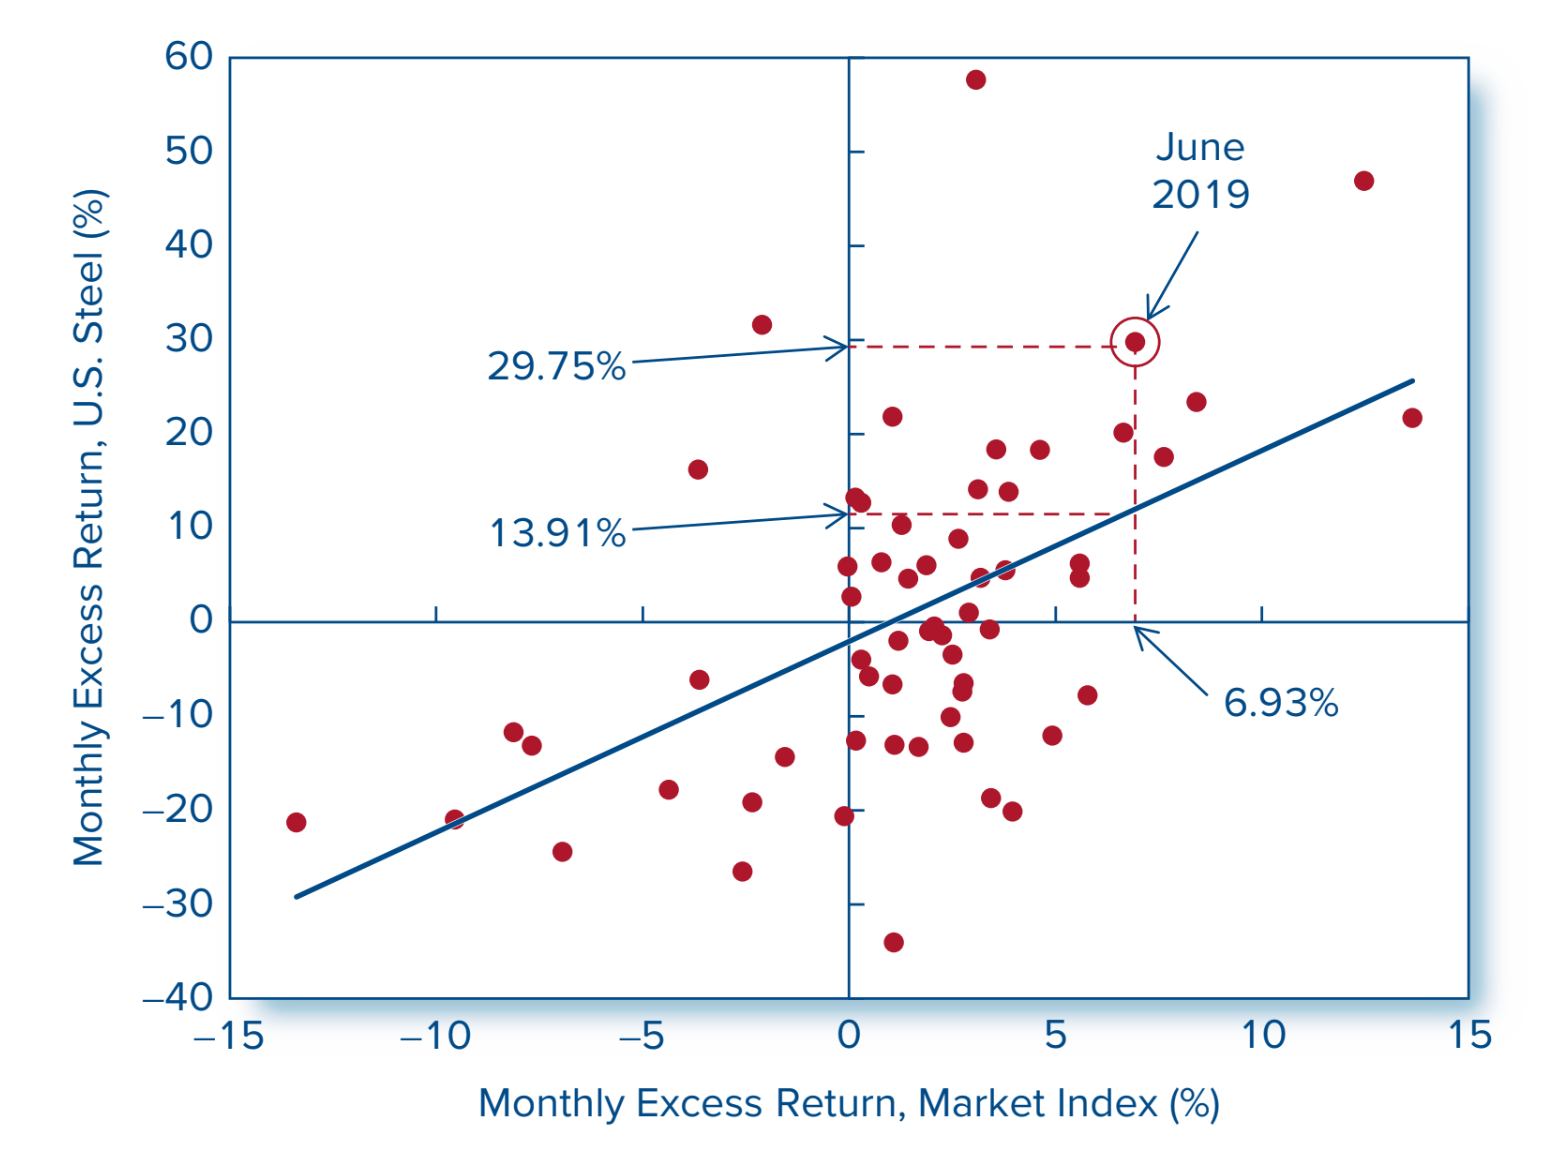
\includegraphics[width=10cm, height=8cm]{./img/8_figura_excesos.png}

La pendiente de la linea de la figura es el coeficiente $\beta$ de la security. Entonces, $\beta$ es la la cantidad por la cual los retornos de
la security aumenta o decrece por cada 1 o 2 porciento de incremento del indice, midiendo la sensibilidad del activo al indice de mercado.
$e_i$(t) es la media 0, o sorpresa, firm-specific en los retornos para un mes $t$, tambien llamado residual. Cuanto mas grande los residuals, tanto negativo como positivo,
 mas amplia es la dispersion de retornos al rededor de la linea de regresion. 
\\

Nacen dos preguntas importantes. (1) Cual es la relacion esperada entre el beta de un activo y su retorno esperado? 
(2) Cual es el alpha que esperamos cuando los mercados estan en equilibrio?.
\\

\textbf{The Regression Equation of the Single-Index Model}
\\

Tomando $E(e_i)$ = 0, obtenemos la relacion  beta-retornos con del single-index model:

\[
\begin{aligned}
E(R_i) = \alpha_i + \beta_i E(R_M)
\end{aligned}
\]
La segunda parte, nos dice que el premium(compensación adicional que un inversor espera obtener por asumir el riesgo de un activo en lugar de invertir en un activo libre de riesgo.) 
de un security-risk, esta dado por el riesgo premium del indice.
\\

\textbf{Risk and Covariance in the Single-Index Model}
\\
Derivamos los siguietnes elementos de la input list de optimizacion de porfolio de markowitz a los parametros del index model.

\begin{flalign*}
& \textbf{Total risk} = \textbf{Systematic risk} + \textbf{Firm-specific risk} & \\
& \sigma_i^2 = \beta_i^2 \sigma_M^2 + \sigma_{\varepsilon_i}^2 \quad \text{(compare to Equation 8.3)} & \\
& \textbf{Covariance} = \textbf{Product of betas} \times \textbf{Market-index risk} & \\
& \mathrm{Cov}(r_i, r_j) = \beta_i \beta_j \sigma_M^2 \quad \text{(compare to Equation 8.4)} & \\
& \textbf{Correlation} = \textbf{Product of correlations with the market index} & \\
& \mathrm{Corr}(r_i, r_j) = \frac{\beta_i \beta_j \sigma_M^2}{\sigma_i \sigma_j} & \\
& = \frac{\beta_i \sigma_M}{\sigma_i} \times \frac{\beta_j \sigma_M}{\sigma_j} & \\
& = \mathrm{Corr}(r_i, r_M) \times \mathrm{Corr}(r_j, r_M) &
\end{flalign*}

\section{Arbitrage Pricing Theory and Multifactor Models of Risk and Return - Capitulo 10}
El model de factores descompone los retornos en sistematicos e idiosincraticos. Existe un problema de tomar
al riesgo sistematico con un unico factor cuando no lo es. Se menciona el riesgo sistematico como la fuentes de
 la prima de riesgo. Existen otras fuentes de riesgo como tasas de interes, inflacion, etc. Entonces, otra representacion de 
 riesgo sistematico puede ser un buen refinamiento del model de unico factor y nos permite tener un mayor entendimiento de los retornos.

\end{document}